\documentclass{standalone}
\usepackage{tikz}
\usetikzlibrary{patterns, positioning}
\usepackage[sfdefault]{ClearSans} %% option 'sfdefault' activates Clear Sans as the default text font
\usepackage[T1]{fontenc}

\begin{document}
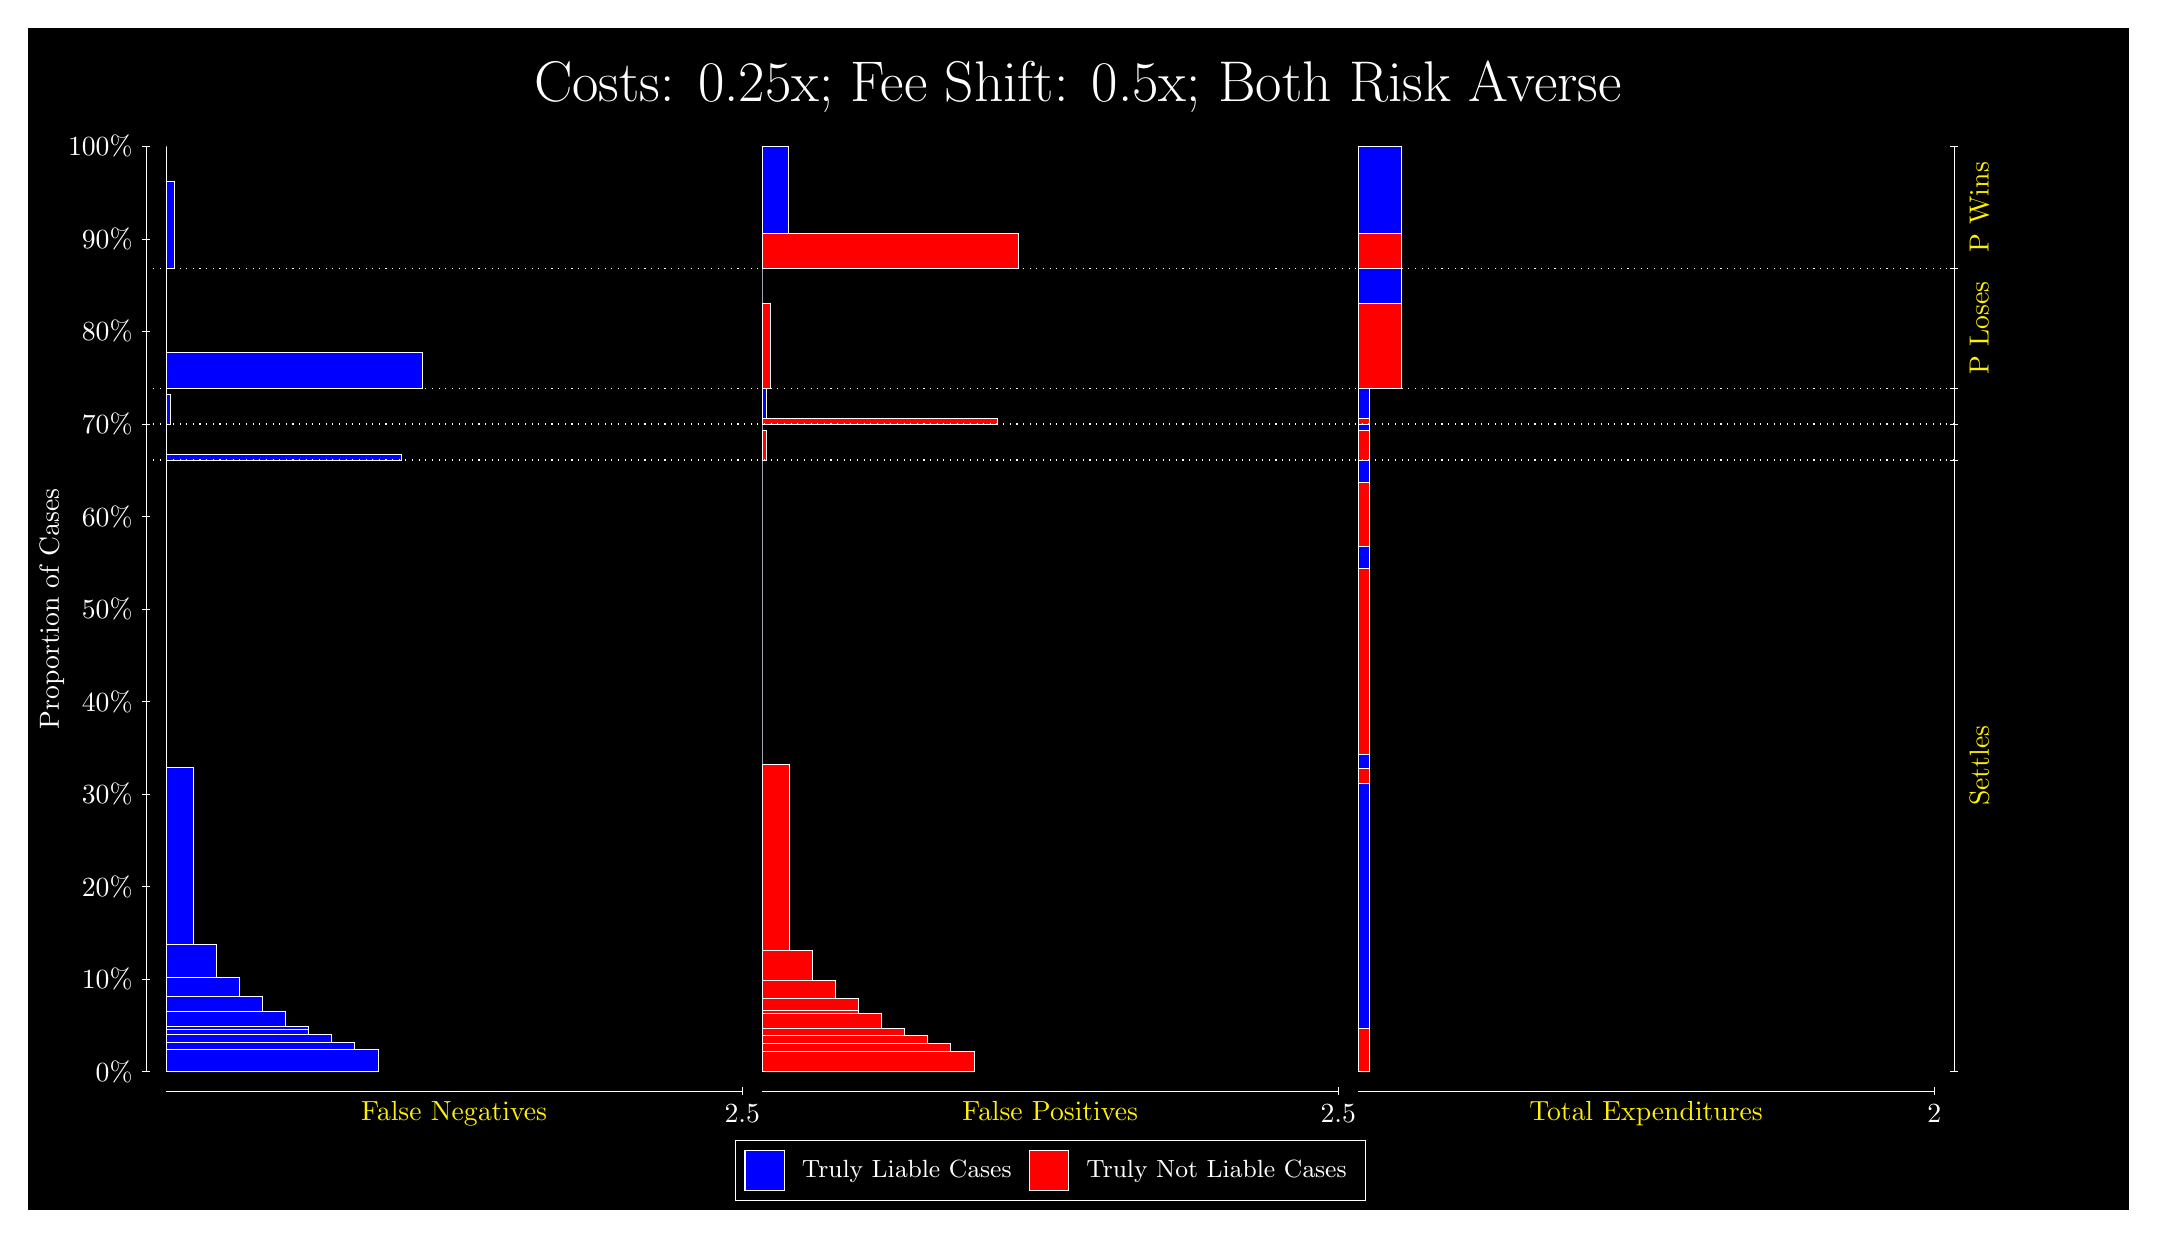
\begin{tikzpicture}
\draw[fill=black] (0,0) rectangle (26.667,15);
\draw[text=white] (0,13.5) rectangle (26.667,15) node[midway] {\huge Costs: 0.25x; Fee Shift: 0.5x; Both Risk Averse};
\draw[white, very thin] (1.5,1.75) -- (1.5,13.5);
\node[rotate=90, text=white, anchor=center] at (0.3, 7.625) {Proportion of Cases};
\draw[white, very thin] (1.45,1.75) -- (1.55,1.75);
\node[text=white, anchor=east] at (1.45, 1.75) {0\%};
\draw[white, very thin] (1.45,2.925) -- (1.55,2.925);
\node[text=white, anchor=east] at (1.45, 2.925) {10\%};
\draw[white, very thin] (1.45,4.1) -- (1.55,4.1);
\node[text=white, anchor=east] at (1.45, 4.1) {20\%};
\draw[white, very thin] (1.45,5.275) -- (1.55,5.275);
\node[text=white, anchor=east] at (1.45, 5.275) {30\%};
\draw[white, very thin] (1.45,6.45) -- (1.55,6.45);
\node[text=white, anchor=east] at (1.45, 6.45) {40\%};
\draw[white, very thin] (1.45,7.625) -- (1.55,7.625);
\node[text=white, anchor=east] at (1.45, 7.625) {50\%};
\draw[white, very thin] (1.45,8.8) -- (1.55,8.8);
\node[text=white, anchor=east] at (1.45, 8.8) {60\%};
\draw[white, very thin] (1.45,9.975) -- (1.55,9.975);
\node[text=white, anchor=east] at (1.45, 9.975) {70\%};
\draw[white, very thin] (1.45,11.15) -- (1.55,11.15);
\node[text=white, anchor=east] at (1.45, 11.15) {80\%};
\draw[white, very thin] (1.45,12.325) -- (1.55,12.325);
\node[text=white, anchor=east] at (1.45, 12.325) {90\%};
\draw[white, very thin] (1.45,13.5) -- (1.55,13.5);
\node[text=white, anchor=east] at (1.45, 13.5) {100\%};

\draw[white, very thin] (24.457,1.75) -- (24.457,13.5);
\draw[white, very thin] (24.407,1.75) -- (24.507,1.75);
\node[anchor=west] at (24.407, 1.75) {};
\draw[white, very thin] (24.407,9.516) -- (24.507,9.516);
\node[anchor=west] at (24.407, 9.516) {};
\draw[white, very thin] (24.407,9.9736) -- (24.507,9.9736);
\node[anchor=west] at (24.407, 9.9736) {};
\draw[white, very thin] (24.407,10.43) -- (24.507,10.43);
\node[anchor=west] at (24.407, 10.43) {};
\draw[white, very thin] (24.407,11.953) -- (24.507,11.953);
\node[anchor=west] at (24.407, 11.953) {};
\draw[white, very thin] (24.407,13.5) -- (24.507,13.5);
\node[anchor=west] at (24.407, 13.5) {};

\draw[white, very thin, fill=blue] (1.75,1.75) rectangle (4.4397,2.034);
\draw[white, very thin, fill=blue] (1.75,2.034) rectangle (4.1469,2.1208);
\draw[white, very thin, fill=blue] (1.75,2.1208) rectangle (3.8542,2.2267);
\draw[white, very thin, fill=blue] (1.75,2.2267) rectangle (3.5614,2.2825);
\draw[white, very thin, fill=blue] (1.75,2.2825) rectangle (3.5614,2.3226);
\draw[white, very thin, fill=blue] (1.75,2.3226) rectangle (3.2687,2.5111);
\draw[white, very thin, fill=blue] (1.75,2.5111) rectangle (2.9759,2.7108);
\draw[white, very thin, fill=blue] (1.75,2.7108) rectangle (2.6832,2.9493);
\draw[white, very thin, fill=blue] (1.75,2.9493) rectangle (2.3904,3.3716);
\draw[white, very thin, fill=blue] (1.75,3.3716) rectangle (2.0976,5.6197);
\draw[white, very thin, fill=red] (1.75,5.6197) rectangle (1.75,9.516);
\draw[white, very thin, fill=blue] (1.75,9.516) rectangle (4.7324,9.5933);
\draw[white, very thin, fill=red] (1.75,9.5933) rectangle (1.75,9.9736);
\draw[white, very thin, fill=blue] (1.75,9.9736) rectangle (1.8049,10.354);
\draw[white, very thin, fill=red] (1.75,10.354) rectangle (1.75,10.43);
\draw[white, very thin, fill=blue] (1.75,10.43) rectangle (5.0069,10.88);
\draw[white, very thin, fill=red] (1.75,10.88) rectangle (1.75,11.953);
\draw[white, very thin, fill=blue] (1.75,11.953) rectangle (1.8598,13.05);
\draw[white, very thin, fill=red] (1.75,13.05) rectangle (1.75,13.5);
\draw[white, very thin, fill=red] (9.3189,1.75) rectangle (12.009,2.0125);
\draw[white, very thin, fill=red] (9.3189,2.0125) rectangle (11.716,2.1026);
\draw[white, very thin, fill=red] (9.3189,2.1026) rectangle (11.423,2.2062);
\draw[white, very thin, fill=red] (9.3189,2.2062) rectangle (11.13,2.3028);
\draw[white, very thin, fill=red] (9.3189,2.3028) rectangle (10.838,2.4883);
\draw[white, very thin, fill=red] (9.3189,2.4883) rectangle (10.545,2.5318);
\draw[white, very thin, fill=red] (9.3189,2.5318) rectangle (10.545,2.6757);
\draw[white, very thin, fill=red] (9.3189,2.6757) rectangle (10.252,2.9062);
\draw[white, very thin, fill=red] (9.3189,2.9062) rectangle (9.9593,3.2957);
\draw[white, very thin, fill=red] (9.3189,3.2957) rectangle (9.6665,5.6463);
\draw[white, very thin, fill=blue] (9.3189,5.6463) rectangle (9.3189,9.516);
\draw[white, very thin, fill=red] (9.3189,9.516) rectangle (9.3738,9.8963);
\draw[white, very thin, fill=blue] (9.3189,9.8963) rectangle (9.3189,9.9736);
\draw[white, very thin, fill=red] (9.3189,9.9736) rectangle (12.301,10.05);
\draw[white, very thin, fill=blue] (9.3189,10.05) rectangle (9.3738,10.43);
\draw[white, very thin, fill=red] (9.3189,10.43) rectangle (9.4287,11.503);
\draw[white, very thin, fill=blue] (9.3189,11.503) rectangle (9.3189,11.953);
\draw[white, very thin, fill=red] (9.3189,11.953) rectangle (12.576,12.402);
\draw[white, very thin, fill=blue] (9.3189,12.402) rectangle (9.6482,13.5);
\draw[white, very thin, fill=red] (16.888,1.75) rectangle (17.025,2.3028);
\draw[white, very thin, fill=blue] (16.888,2.3028) rectangle (17.025,5.4114);
\draw[white, very thin, fill=red] (16.888,5.4114) rectangle (17.025,5.5969);
\draw[white, very thin, fill=blue] (16.888,5.5969) rectangle (17.025,5.7854);
\draw[white, very thin, fill=red] (16.888,5.7854) rectangle (17.025,8.136);
\draw[white, very thin, fill=blue] (16.888,8.136) rectangle (17.025,8.4201);
\draw[white, very thin, fill=red] (16.888,8.4201) rectangle (17.025,9.2275);
\draw[white, very thin, fill=blue] (16.888,9.2275) rectangle (17.025,9.516);
\draw[white, very thin, fill=red] (16.888,9.516) rectangle (17.025,9.8963);
\draw[white, very thin, fill=blue] (16.888,9.8963) rectangle (17.025,9.9736);
\draw[white, very thin, fill=red] (16.888,9.9736) rectangle (17.025,10.05);
\draw[white, very thin, fill=blue] (16.888,10.05) rectangle (17.025,10.43);
\draw[white, very thin, fill=red] (16.888,10.43) rectangle (17.437,11.503);
\draw[white, very thin, fill=blue] (16.888,11.503) rectangle (17.437,11.953);
\draw[white, very thin, fill=red] (16.888,11.953) rectangle (17.437,12.402);
\draw[white, very thin, fill=blue] (16.888,12.402) rectangle (17.437,13.5);
\draw[white, dotted] (1.5,9.516) -- (24.457,9.516);
\draw[white, dotted] (1.5,9.9736) -- (24.457,9.9736);
\draw[white, dotted] (1.5,10.43) -- (24.457,10.43);
\draw[white, dotted] (1.5,11.953) -- (24.457,11.953);
\draw[white, very thin] (1.75,1.5) -- (9.0689,1.5);
\node[text=yellow, anchor=north] at (5.4094, 1.5) {False Negatives};
\draw[white, very thin] (9.0689,1.45) -- (9.0689,1.55);
\node[text=white, anchor=north] at (9.0689, 1.45) {2.5};

\draw[white, very thin] (9.3189,1.5) -- (16.638,1.5);
\node[text=yellow, anchor=north] at (12.978, 1.5) {False Positives};
\draw[white, very thin] (16.638,1.45) -- (16.638,1.55);
\node[text=white, anchor=north] at (16.638, 1.45) {2.5};

\draw[white, very thin] (16.888,1.5) -- (24.207,1.5);
\node[text=yellow, anchor=north] at (20.547, 1.5) {Total Expenditures};
\draw[white, very thin] (24.207,1.45) -- (24.207,1.55);
\node[text=white, anchor=north] at (24.207, 1.45) {2};

\node[text=yellow, centered, rotate=90] at (24.777, 5.633) {Settles};


\node[text=yellow, centered, rotate=90] at (24.777, 11.191) {P Loses};
\node[text=yellow, centered, rotate=90] at (24.777, 12.726) {P Wins};

\draw (12.978300999999998,1.5) node[draw=none] (baseCoordinate) {};
\begin{scope}[align=center]
        \matrix[scale=0.5, draw=white, below=0.5cm of baseCoordinate, nodes={draw}, column sep=0.1cm]{
            \node[rectangle, draw, minimum width=0.5cm, minimum height=0.5cm, fill=blue] {}; &
            \node[draw=none, font=\small, text=white] (B) {Truly Liable Cases}; &
            \node[rectangle, draw, minimum width=0.5cm, minimum height=0.5cm, fill=red] {}; &
            \node[draw=none, font=\small, text=white] (B) {Truly Not Liable Cases}; \\
            };
\end{scope}

\end{tikzpicture}
\end{document}